%%%%%%%%%%%%%%%%%%%%%%%%%%%%%%%%%%%%%%%%%%%%%%%%%%%%%%%%%%%%%
% ECE 445 SENIOR DESIGN TEMPLATE
%%%%%%%%%%%%%%%%%%%%%%%%%%%%%%%%%%%%%%%%%%%%%%%%%%%%%%%%%%%%%
\documentclass[letterpaper,10pt]{article}

%%%%%%%%%%%%%%%%%%%%%%%%%%%%%%%%%%%%%%%%%%%%%%%%%%%%%%%%%%%%%
% The preamble starts here.
% You can add other packages that you want to use by using
% \usepackage command in the preamble.
% However, DO NOT change the settings that are already placed
% below unless you really know what you are doing.
%%%%%%%%%%%%%%%%%%%%%%%%%%%%%%%%%%%%%%%%%%%%%%%%%%%%%%%%%%%%%

% some commonly used packages
\usepackage{siunitx}
\usepackage{graphicx}
\usepackage{color,soul}
\usepackage{amsmath}
\usepackage{amsthm}
\usepackage{amsfonts}
\usepackage{setspace}
\usepackage{longtable}
\usepackage{url}
\usepackage{float}
\usepackage{caption}
\usepackage{booktabs}  % professional-looking tables
\usepackage{multicol} %used for getting multicolumn without page-break
\usepackage{multirow}	% multi-row tables
\usepackage{array}		% define column format of a table
\usepackage[colorlinks=true,linkcolor=black,citecolor=black]{hyperref}
\usepackage[top=1in, bottom=1in, left=1in, right=1in]{geometry}% set the page margins to 1 inch

% use the fancyhdr package to maintain the format of the page numbers,
% which is useful when the text color is changed
\usepackage{fancyhdr}
\fancyhf{}
\renewcommand{\headrulewidth}{1pt}
\renewcommand{\footrulewidth}{0pt}
\fancyfoot[C]{\textcolor{black}{\thepage}}
\fancyhead[L]{
\includegraphics[width=2cm]{University-of-Illinois-logo.jpg}}
\fancyhead[R]{\small{Infantry I.F.F. Design Review - Meyers \& Prince}}

% paralist provides extended list environments
\usepackage{paralist}
\setlength{\plitemsep}{0pt}

% define the color for section and subsection titles
\usepackage{xcolor}
\definecolor{titlecolor}{RGB}{31,73,125}
\definecolor{subtitlecolor}{RGB}{79,129,189}

% change the style of the section and subsection titles
\usepackage{titlesec}
\titleformat{\section}{\color{titlecolor}\Large\bf}{\color{titlecolor}\thesection}{0.8em}{}
\titleformat{\subsection}{\color{subtitlecolor}\large\bf}{\color{subtitlecolor}\thesubsection}{1em}{}
\titleformat{\subsubsection}{\color{subtitlecolor}\normalsize\bf}{\color{subtitlecolor}\thesubsubsection}{1.2em}{}
\titlespacing{\section}{0pt}{0em}{0em}
\titlespacing{\subsection}{6pt}{0em}{0em}
\titlespacing{\subsubsection}{12pt}{0em}{0em}



% change the style of the table of contents
\usepackage{titletoc}
\titlecontents{section}[1.5em]{}{\contentslabel{1.5em}}{\hspace*{-1.5em}}{\titlerule*[0.5pc]{.}\contentspage}
\titlecontents{subsection}[3em]{}{\contentslabel{2.1em}}{\hspace*{-2.1em}}{\titlerule*[0.5pc]{.}\contentspage}
\titlecontents{subsubsection}[5.1em]{}{\contentslabel{2.7em}}{\hspace*{-2.7em}}{\titlerule*[0.5pc]{.}\contentspage}

% command for centering texts in a fixed width table cell
\newcommand{\centpcol}{\leftskip\fill \rightskip\fill}

% command for setting the style of the appendix titles
\newcommand{\setappenstyle}{
	\titleformat{\section}{\color{titlecolor}\Large\bf}{\color{titlecolor}Appendix \Alph{section}}{0.8em}{}
	\titlecontents{section}[0em]{}{Appendix \thecontentslabel \hspace{1em}}{}{\titlerule*[0.5pc]{.}\contentspage}
}

\makeatletter
\newcommand{\skipitems}[1]{%
	\addtocounter{\@enumctr}{#1}%
}

% define the style of the title of the paper
\newcommand{\thetitle}[1]{\title{\begin{huge}{\bf #1}\end{huge} \color{subtitlecolor}\rule[25pt]{\textwidth}{1pt}}}

% define the style of the author
\newcommand{\theauthor}[3]{
	\author{\vspace{.4in}\\
	\textcolor{black}{By}\\
	#1
	\vspace{1in}\\
	\textcolor{black}{ECE 445 Design Review -} #2\\
	\textcolor{black}{TA:} #3
	\vspace{1in}}
}

% define the style of figure's caption
\newcommand{\figcap}[1]{
	\captionsetup{format=plain,font={small,color=subtitlecolor,singlespacing},margin={0pt,0pt}}
	\caption{\textcolor{subtitlecolor}{#1}}
	\vspace{-5pt}
}

% define the style of table's caption
\newcommand{\tablecap}[1]{
	\captionsetup{format=plain,font={bf,normalsize,singlespacing,color=black},margin={0pt,0pt}}
	\caption{\textcolor{black}{#1}}
	\vspace{-5pt}
}


\newcommand{\buildtoc}{
	\clearpage
	\singlespacing
	\tableofcontents
	\onehalfspacing
}

% set indentations and the space between paragraghs
\setlength{\parindent}{0pt}
\setlength{\parskip}{8pt}

\setcounter{secnumdepth}{4}

\titleformat{\paragraph}
{\normalfont\small\bfseries\color{subtitlecolor}}{\theparagraph}{1em}{}
\titlespacing*{\paragraph}
{18pt}{3.25ex plus 1ex minus .2ex}{1.5ex plus .2ex}

%%%%%%%%%%%%%%%%%%%%%%%%%%%%%%%%%%%%%%%%%%%%%%%%%%%%%%%%%%%%%
% PREAMBLE ENDS HERE, DOCUMENT STARTS BELOW
%%%%%%%%%%%%%%%%%%%%%%%%%%%%%%%%%%%%%%%%%%%%%%%%%%%%%%%%%%%%%

\begin{document}

% don't change these
\pagestyle{empty}
\doublespacing

% put the title of your project here. DO NOT include the brackets.
\thetitle{{I.F.F. (Identification Friend or Foe) System}}

% put your names here. seperate by \\. DO NOT include the brackets.
\theauthor{
	{Eric Meyers (emeyer7)}\\
	{Noah Prince (nprince2)}\\
}
{ % put the semester info here. DO NOT include the brackets.
	{Spring 2016}
}
{ % put your TA's name here. DO NOT include the brackets.
	{Braedon Salz}
}

% put the date and project number here. DO NOT include the brackets.
\date{
{March 2nd, 2016}\\
Project No. 11
\clearpage
}

% don't change these
\maketitle
\pagestyle{fancy}
\begin{spacing}{1.15}


% build the table of contents. 
\color{black}
\buildtoc
\pagenumbering{gobble}
\clearpage
\setcounter{page}{1}
\pagenumbering{arabic}

%SECTION - Introduction
\section{Introduction}
\subsection{Statement of Purpose}
There have been several friendly fire incidents in recorded military history, accounting for an estimated 2\% to 20\% of all casualties in battle\textsuperscript{\cite{USArmy}}. Using attire to identify friend vs enemy is problematic in situations when both sides are clad in the same camouflage pattern, or are obscured by obstacles.

The purpose of this project is to create a system that quickly and accurately identifies friendly targets among military personnel on foot. Similar systems exist for aircraft, however not many exist for infantry.

The idea is to develop a two-way communication system so that when a soldier aims their weapon in the direction of a friendly target, they will receive notification through an LED that the target is, indeed, friendly and not an enemy. Throughout this document the infantry unit with the weapon will be referred to the "friendly interrogator" and the target will  be referred to as the "friendly target". 

This communication protocol can be 
\subsection{Objectives}
\subsubsection{Goals and Benefits}
\begin{itemize}
	\item Reduce number of friendly fire accidents during combat \textsuperscript{\cite{Garrison}}
	\item Reduce number of misfires accidents during combat \textsuperscript{\cite{Garrison}}
	\item Notify friendly personnel location of particular friendly target when aiming
	\item Other applications including but not limited to:
	\begin{itemize}
		\item Paintball or Airsoft
		\item Arcade Laser Tag
	\end{itemize}
\end{itemize}
\subsubsection{Functions and Features}
\begin{itemize}
	\item Laser diode on friendly interrogator to transmit unique I.D. of friendly interrogator.
	\item Photodiodes on friendly target to detect unique I.D. and verify it is a valid signal.
	\item R.F. Transmitter on friendly target to send acknowledgement back to interrogator.
	\item R.F. Receiver on friendly interrogator to verify that the target is friendly.
	\item LED on friendly interrogator to indicate to the operator the status of the target.
\end{itemize}
\clearpage

%SECTION - Design
\section{Design}
%Subsection - Block Diagrams
\subsection{Block Diagrams and Descriptions}
\subsubsection{System Overview}
The following figure represents the system as a whole, including both the friendly interrogator unit and the friendly target unit. Both units will be expanded upon in further detail below.
\begin{figure} [H]
	\centering
	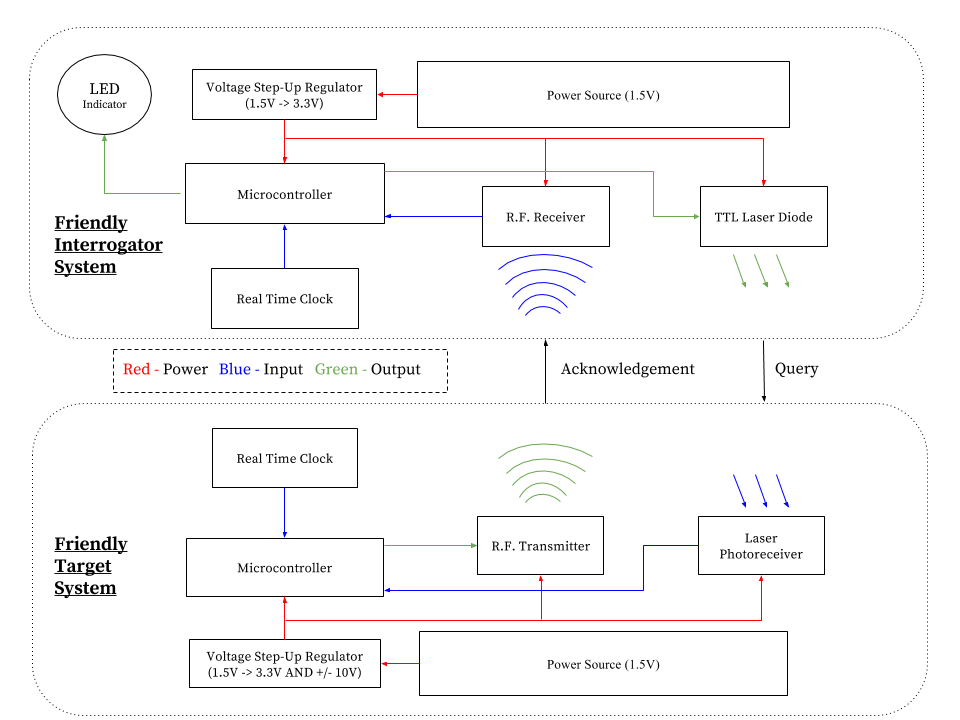
\includegraphics[scale=0.45]{System_Block_Diagram.png}
	\caption{System Block Diagram\label{fig:system-block-diagram}}
\end{figure}

%DESIGN - FRIENDLY INTERROGATOR UNIT
\subsubsection{Friendly Interrogator Unit} \label{section-friendly-interrogator-design}
The following diagram shows the friendly interrogator unit \textit{only}. The interconnections in red represent power, interconnections in blue represent input to a block and interconnections in green represent output to a block. These inputs and outputs are described below under each block description.
\begin{figure} [H]
\centering
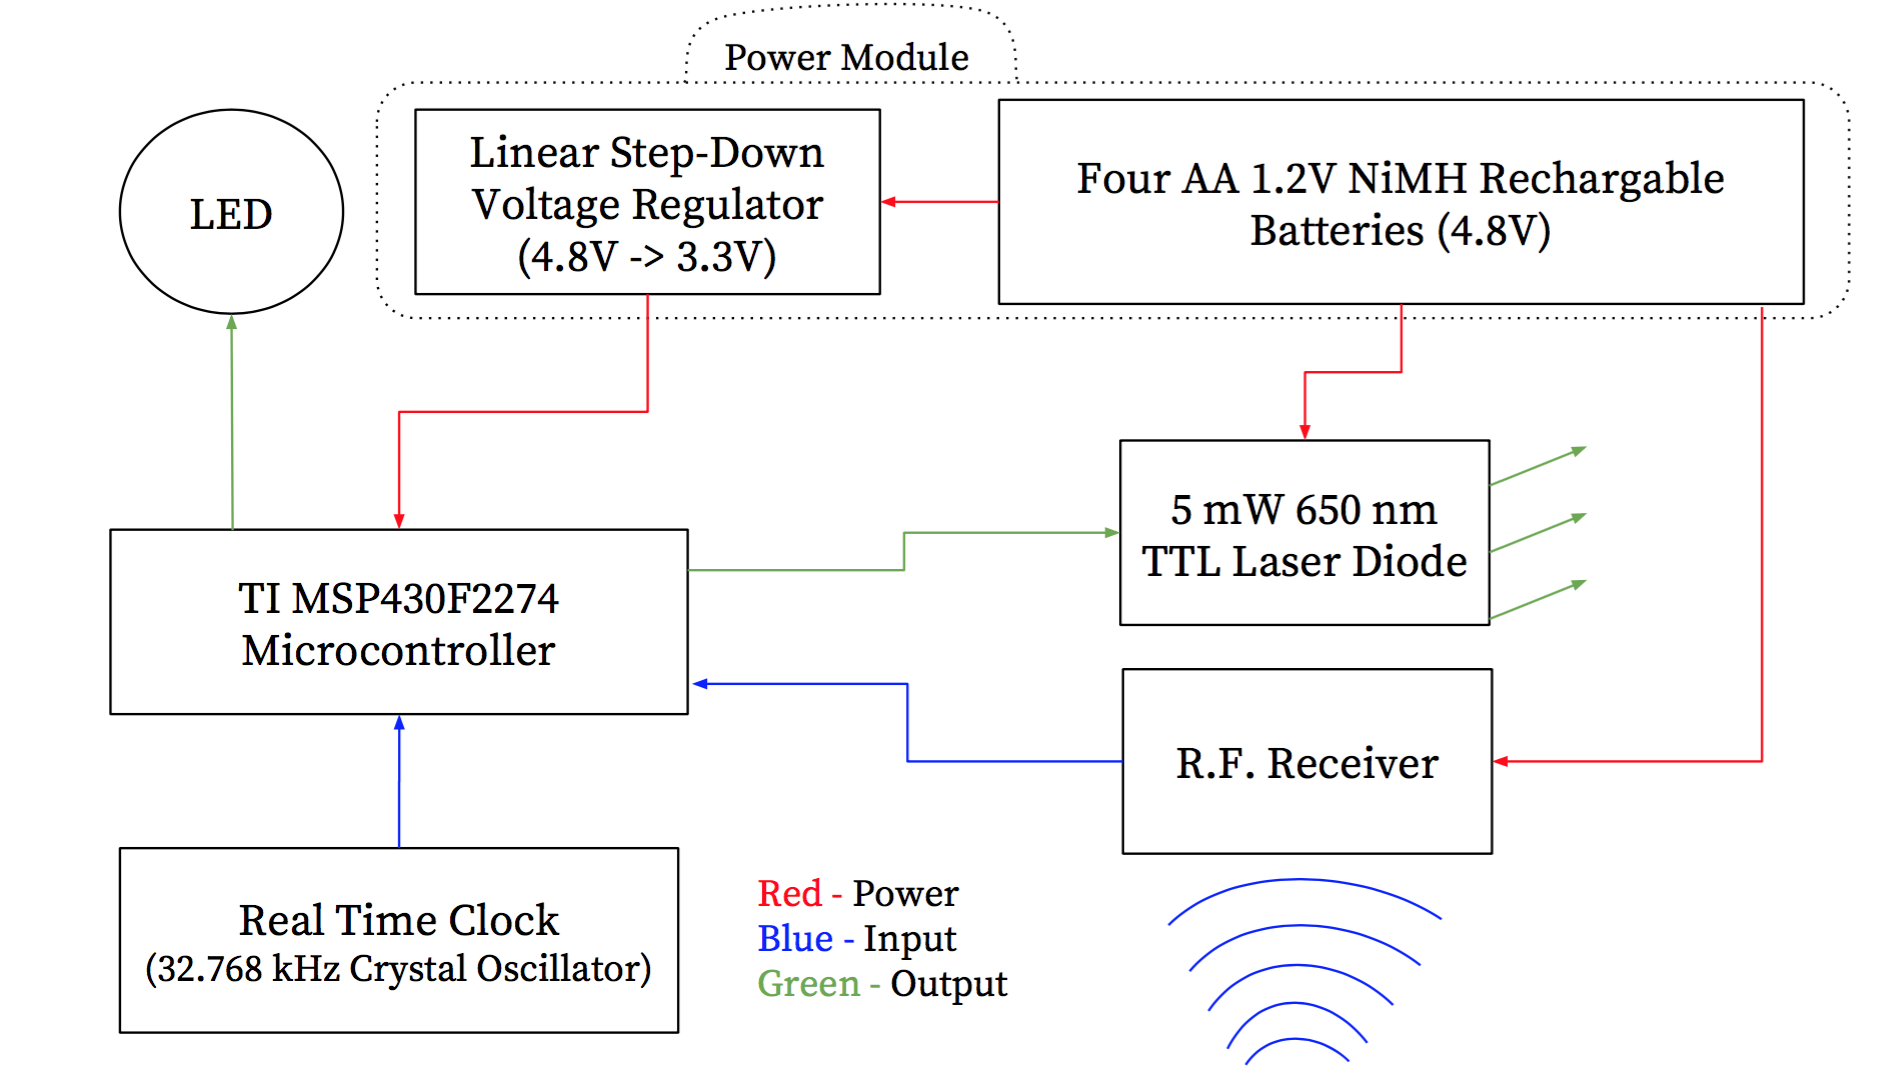
\includegraphics[scale=0.5]{Friendly_Interrogator_Block_Diagram.png}
\caption{Block Diagram of Friendly Interrogator Unit\label{fig:friendly-interrogator-block}}
\end{figure}

\normalsize\textbf{Power Module} \\
Power-In, ,  N/A \\
Power-Out: MSP430 Microcontroller, 5mW Laser Transmitter, R.F. Receiver/Decoder, LED Indicator \\
Input(s): N/A\\
Output(s): N/A

The power module will consist of a single standard alkaline AA battery (no specific brand/part name is necessary) which will lead into a Skyworks AAT1217 DC-DC step-up voltage converter. This will step the voltage up to 3.3V with a maximum current output of 100 mA which is sufficient enough to power the MCU, laser transmitter, and the R.F. receiver. Please refer to Section \ref{section-simulations-calculations} for these calculations regarding power delivery to this unit and resistor/capacitor/inductor part selection. 

As noted on the block diagram, in between the power module and the R.F. receiver/laser transmitter, there is a switch to control the power given to these two modules. This switch exists for two reasons: (1) to decrease power consumption and (2) to limit the amount of time the laser transmitter is sending data. This design choice will be expanded upon in Section \_\_\_.

The circuit to operate the DC-DC step-up converter is shown in Figure \ref{fig:aat1217-voltage-converter-circuit}. \\



The battery will be mounted to the PCB a standard AA through-hole PCB battery mount shown in Figure \ref{fig:pcb-battery-mount}. However, this will be omitted from the circuit schematic for simplilcity purposes. During the construction of the PCB the team will have to create the 
\begin{figure} [H]
	\centering
	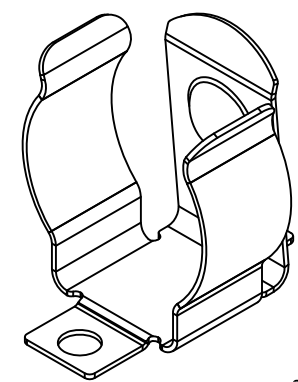
\includegraphics[scale=0.4]{PCB_Battery_Mount.png}
	\caption{PCB Battery Mount\label{fig:pcb-battery-mount}}
\end{figure}

\normalsize\textbf{MSP430 Microcontroller} \\
Power-In: 3.3V (from Voltage Converter Output) \\
Power-Out: N/A \\
Input(s): R.F. Receiver/Decoder Data-Out, 8-Pin DIP Switch,  Real Time Clock (32.768kHz Crystal) \\
Output(s): LED, 5mW 650nm Laser Diode

The team chose to work with an T.I. MSP430F2274 Microcontroller Unit \textsuperscript{\cite{MSP430F2274}} due to its compiler simplicity, its availability in the ECE445 Senior Design Labs (available inventory) and the number of GPIO Pins on board (compared to other options, this model had several I/O pins and was the least expensive). Compared to many other MCUs on the market, the MSP430 is relatively well documented and there exist several support forums on the internet to assist the team throughout the duration of the project.

The board requires a 3.3V power supply to both the DV\textsubscript{cc} (pin 2) and AV\textsubscript{cc} (pin 16) which is why the voltage regulator is necessary as stated in the previous section. 

As stated above, the input the MSP430 MCU will be the R.F. receiver/decoder signal, the 8-pin DIP switch, and the real time clock.

The R.F. receiver/decoder signal will be the acknowledgment sent from the friendly target. These outputs from the receiver/decoder will be fed into pins 20 - 27 on the MCU. This cooresponds to 8 bits of data the MCU will be receiving from the friendly interrogator.

The 8-pin DIP switch, which is the unique I.D. of the friendly interrogator, will be fed into pins 31 -38 on the MCU. 

The 5 mW laser will be fed into pin 17 of the MCU to control the modulation of the signal to send the unique I.D. to the friendly target. 

This unique I.D. provided by the DIP switch will be used in conjunction with the output pin to the laser transmitter to create a "laser pulse" that sends the data of the I.D. to the friendly target. This will be explained in more detail in section \hl{BLAHFUCKINGBLAH}.

\hl{Progr}

The above descriptions can be summarized with Table \ref{tab:msp430-pin-assignments} below. Each pin/label is listed with the description of the input or output. The red rows indicate that the pin is a power/ground line, the blue rows indicate that the pin is an input \textit{to} the MCU and the green rows indicate that the pin is an output \textit{from} the MCU. 

\begin{table} [H]
	\centering
	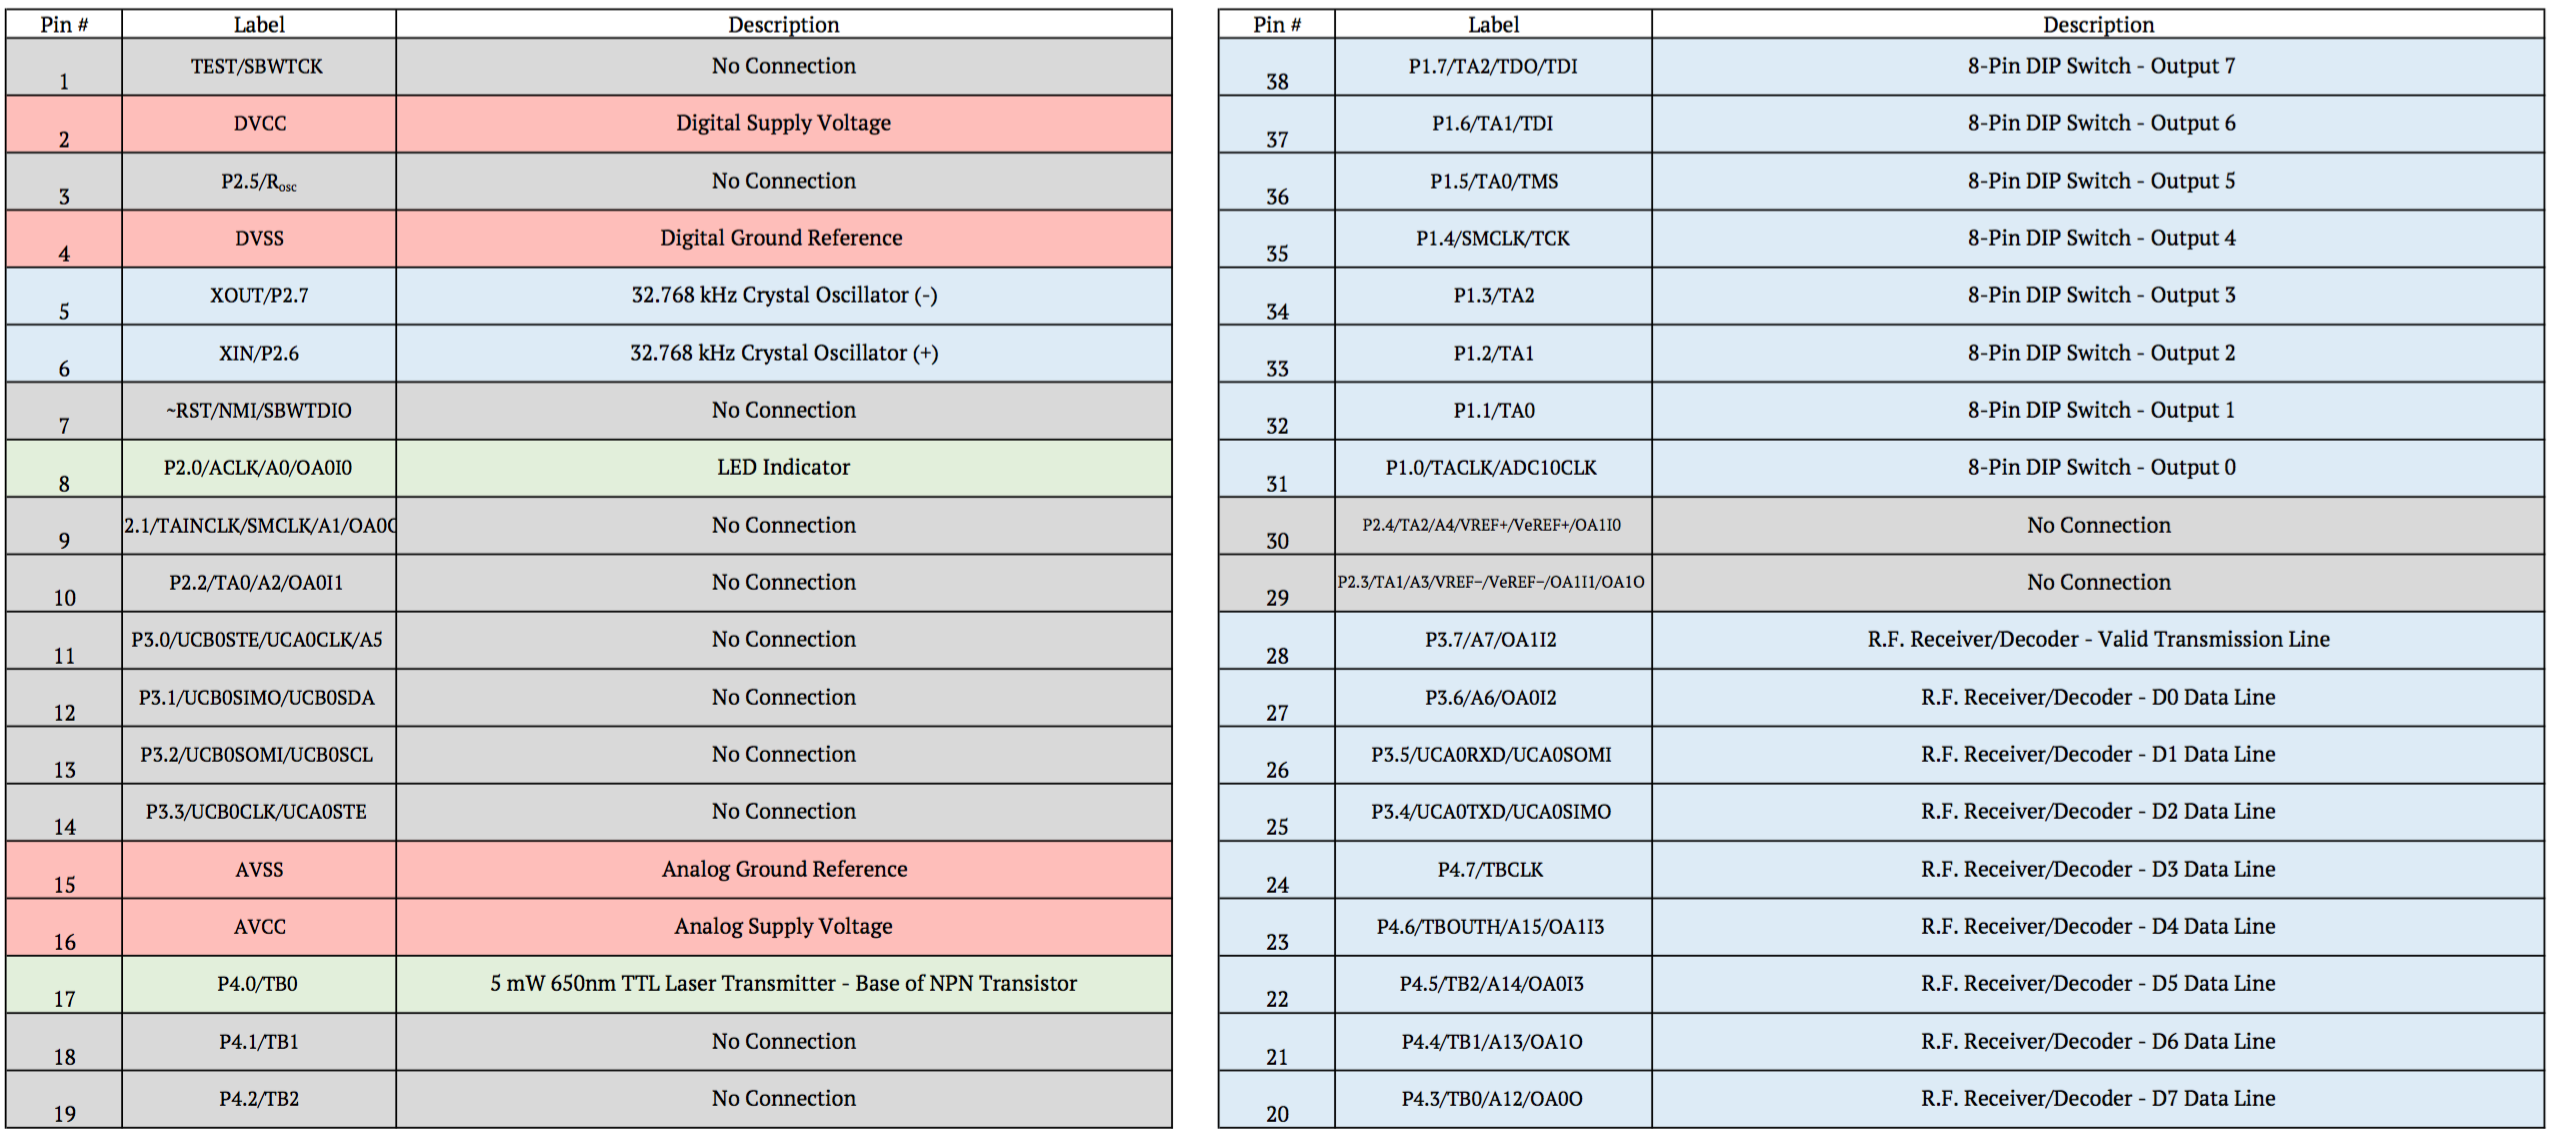
\includegraphics[scale=0.37]{MSP430_Pin_Assignments.png}
	\caption{Pin Layout Table\label{tab:msp430-pin-assignments}}
\end{table}

Please refer to Section \ref{section-functionality} to view in-depth discussion about the functionality of the MSP430F2274 Microcontroller Unit and how it will be used throughout this project.

\normalsize\textbf{Real Time Clock}\\
Power-In: N/A \\
Power-Out: N/A \\
Input(s): N/A \\
Output(s): MSP430 Microcontroller

The real time clock is necessary for the verification of the acknowledgement signal sent by the R.F. transmitter on the friendly target unit. It will operate using a 32.768 kHz Crystal Oscillator (as recommended by T.I. \textsuperscript{\cite{RTC-Implementation}}) with an accuracy of +/- 20 PPM (Parts Per Million - deviates between 32.7673 kHz and 32.7687 kHz). It will be used in conjunction with the real time clock library provided by T.I. \hl{INSERT REFERENCE HERE}.

\normalsize\textbf{Laser Diode}\\
Power-In: 3.3V (from Voltage Converter Output) \\
Power-Out: N/A \\
Input(s): MSP430 Microcontroller
Output(s):  5mW 650nm laser signal containing unique I.D. of interrogator 

For safety reasons, the maximum allowable power for the laser diode is $5mW$; which registers as a Class IIIa laser. The laser diode must also fall in the visible range, so that it will trigger a person's blinking reflex before eye damage occurs. Specifically, the team will use a red ($650nm$) laser. See section \ref{section-safety-ethics} for more on safety of the laser. 

The team will use a 5 mW 650 nm TTL laser transmitter to transmit the unique I.D. (as specified by the 8-pin DIP switch) to the friendly target. This laser will operate on 3.3V at 25mA so a 1.3$\Omega$  resistor is necessary to drop the current being supplied to the diode down to this threshold. 

To save cost and time, the team will be purchasing an adjustable focus laser. This laser will allow for optical adjustments to achieve the beam diameter at all required distances. The team will ensure the purchased laser meets these requirements, and will adjust the lens if necessary. 

\normalsize\textbf{R.F. Receiver/Decoder} \\
Power-In: 3.3V (from Voltage Converter Output) \\
Power-Out: N/A \\
Input(s): 8-Pin DIP Switch\\
Output(s): MSP430 Microcontroller

A Linx 315 MHz KH3 Series R.F. Receiver/Decoder will be used for this project along with a Linx 315-SP Splatch PCB Mounted Antenna. Some important values that were used in the selection process of this part are listed in Table \ref{tab:rf-receiver-important-values}

\begin{table}[htbp]
	\centering
	\begin{tabular}{c|c}	% ccccccc indicates 7 center aligned columns
		\toprule	% top separator
		Parameter & Typical Value \\
		\midrule
		Operating Voltage & 3.3V\\
		Supply Current & 5.9mA\\
		Receiver Frequency & 315 MHz \\ 
		Receiver Sensitivity & -116 dB \\
		R.F. Input Impedance & 50 $\Omega$ \\
		Datarate & 100 bps - 10,000 bps  \\
		Receiver Turn-On Time & 7.0 ms  \\
		\bottomrule	% bottom separator
	\end{tabular}%
	\caption{Linx 315 MHz KH3 R.F. Receiver}
	\label{tab:rf-receiver-important-values}	% this is the label given to the table that can be referenced using \ref{tab:Exp1Part1_7}
\end{table}%

Important values to note are the R.F. input impedance, the receiver frequency, and the receiver sensitivity. The input impedence is stating it requires the entire R.F. receiver system to be matched at 50 $\Omega$. This requires the trace on the PCB from the receiver to the antenna to also be at a 50 $\Omega$ impedence. The frequency and sensitivity affect the range of the receiver/transmitter pair and this calculation along with the PCB trace-width calculation can be found in Section \ref{section-simulations-calculations}.

The decoder provides very important functionality and simplicity to the system. There are a total of 10 address lines on the decoder that must match up to the cooresponding transmitting encoder. The lines do not output data through the data-out lines if the address lines do not match up. The team decided to make use of these lines and wire them up to a 8-pin DIP switch so that the operator can choose their unique interrogator I.D. Therefore only 8 out of the 10 address lines on the encoder will be used and the top two most significant bits will be grounded (lines A9 and A10).

As stated before this identification number will be fed into the MCU also and it will determine what the 5mW laser transmitter will send out to the friendly target. This process will be explained in Section \ref{section-functionality}.

%DESIGN - FRIENDLY TARGET UNIT
\subsubsection{Friendly Target Unit}

\begin{figure} [H]
	\centering
	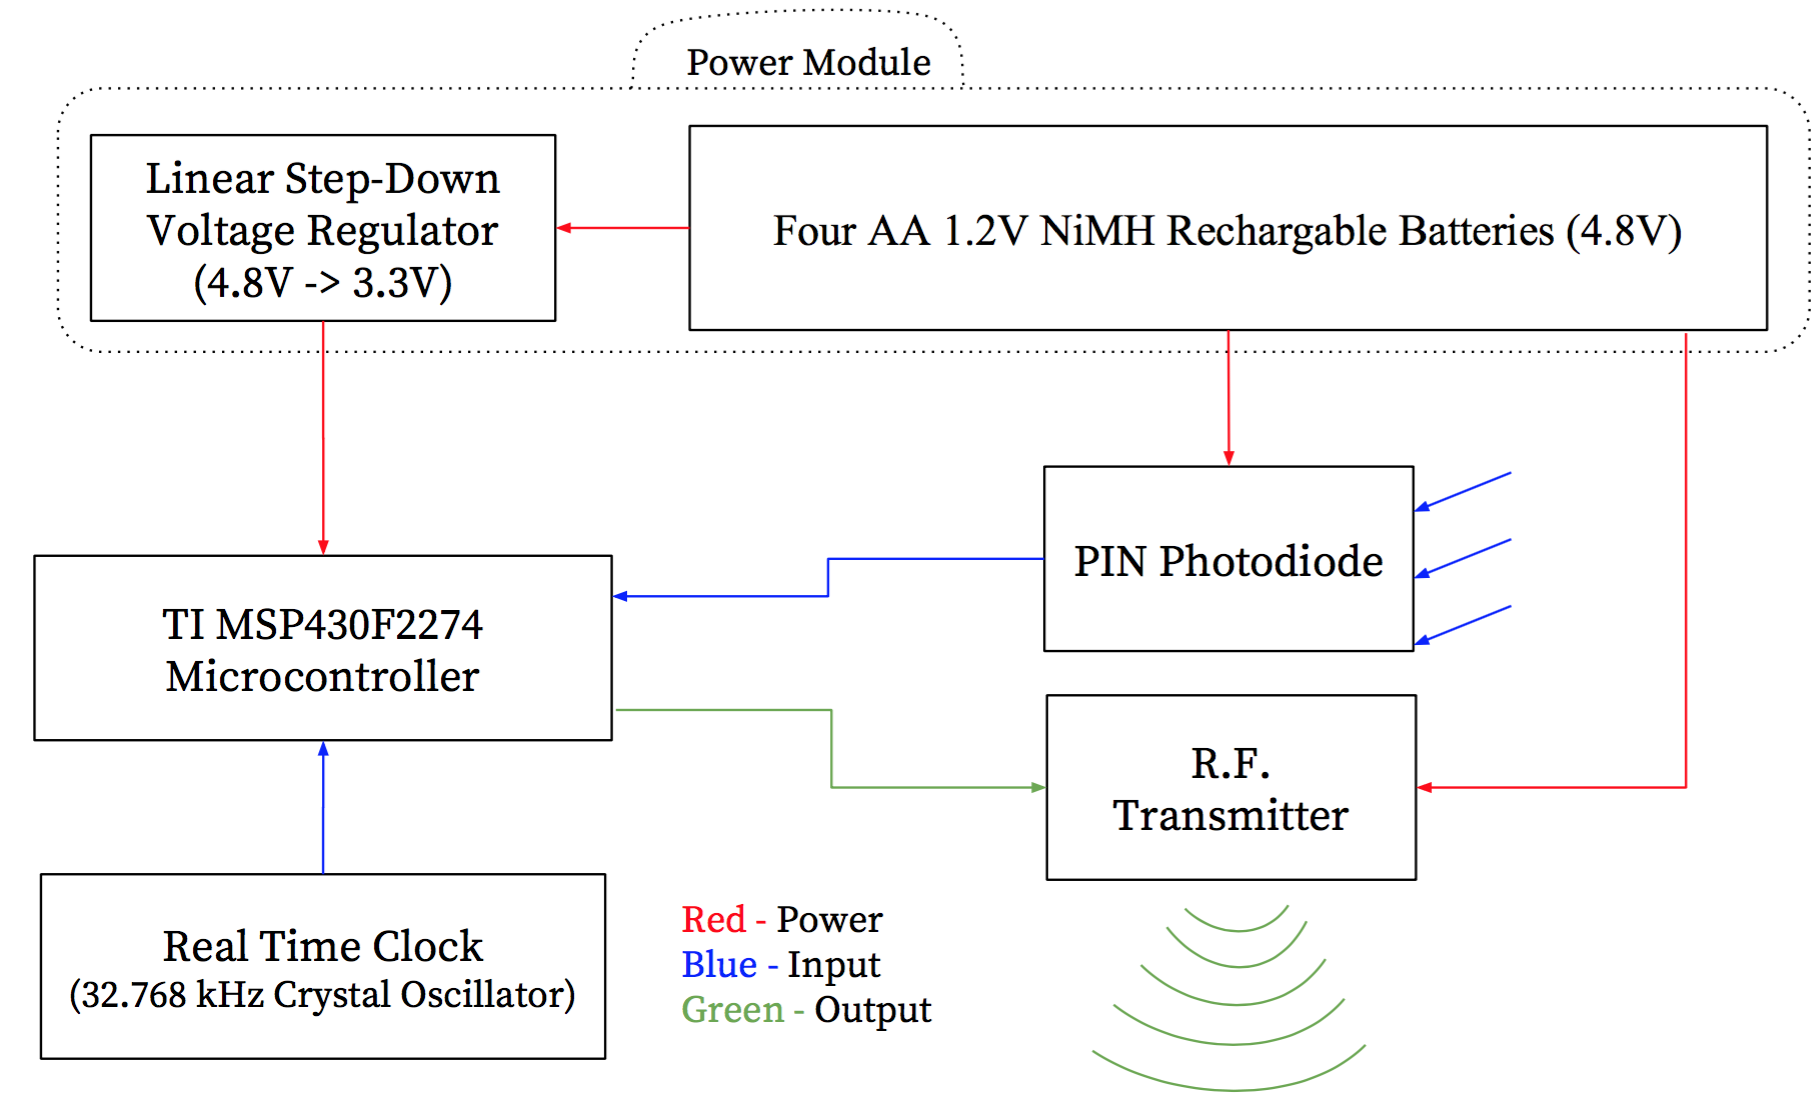
\includegraphics[scale=0.50]{Friendly_Target_Block_Diagram.png}
	\caption{Block Diagram of Friendly Target System\label{fig:friendly-target-block}}
\end{figure}

\normalsize\textbf{Power Module} \\
Power-In: N/A\\
Power-Out: \\
Input(s): \\
Output(s):

The power module on board the Friendly Target Unit will be the same as the Friendly Interrogator Unit. Th Please reference that section to get all details pertaining to the power module.


\normalsize\textbf{Microcontroller} \\
Power-In: \\
Power-Out:\\
Input(s):\\
Output(s):\\
\hl{INDICATE WHICH PINS ARE ACTIVE AND NOT}

\normalsize\textbf{Real Time Clock} \\
Power-In: \\
Power-Out: \\
Input(s): \\
Output(s):

The Real Time Clock on board the Friendly Target Unit will be the same as the Friendly Interrogator Unit. Please reference that section to get all details pertaining to the Real Time Clock.

\normalsize\textbf{Photoreceiver}\\
Power-In: N/A \\
Power-Out: N/A \\
Input(s): Laser Transmitter \\
Output(s): MCU

A network of four photodiodes mounted on the friendly target will report incoming laser signals to the MCU. The photodiode signals will be boosted via an operational amplifier, and passed through a low-pass filter. The $40kHz$ signal that passes through the filter will be sampled and processed by the MCU. 

For a detailed analysis of the choice of the photodiodes, see section \ref{section-tolerance-analysis}

\normalsize\textbf{R.F. Transmitter}\\
Power-In: \\
Power-Out: \\ 
Input(s): \\ 
Output(s):

A Linx 315 MHz LR Series R.F. Transmitter will be used for this project along with a Linx 315-SP Splatch PCB Mounted Antenna. This is an identical setup to the receiver end on the friendly interrogator unit as discussed before.  

\begin{table}[htbp]
	\centering
	\begin{tabular}{c|c}	% ccccccc indicates 7 center aligned columns
		\toprule	% top separator
		Parameter & Typical Value \\
		\midrule
		Transmit Frequency & 315 MHz \\ 
		Output Power & 4 dB \\
		Data Rate & 10,000 bps \\
		R.F. Output Impedance & 50 $\Omega$ \\
		Transmitter Turn-On Time & 1.0 ms  \\
		\bottomrule	% bottom separator
	\end{tabular}%
	\caption{Notable Datasheet Values for Linx 315 MHz LR R.F. Transmitter}
	\label{tab:table2}	% this is the label given to the table that can be referenced using \ref{tab:Exp1Part1_7}
\end{table}



%Subsection - Circuit Schematics
\subsection{Circuit Schematics}

\subsubsection{Friendly Interrogator Unit}
The circuit schematic is shown below for the Friendly Interrogator Subsystem.
\hl{INSERT OVERALL CIRCUIT SCHEMATIC HERE}
\begin{figure} [H]
	\centering
	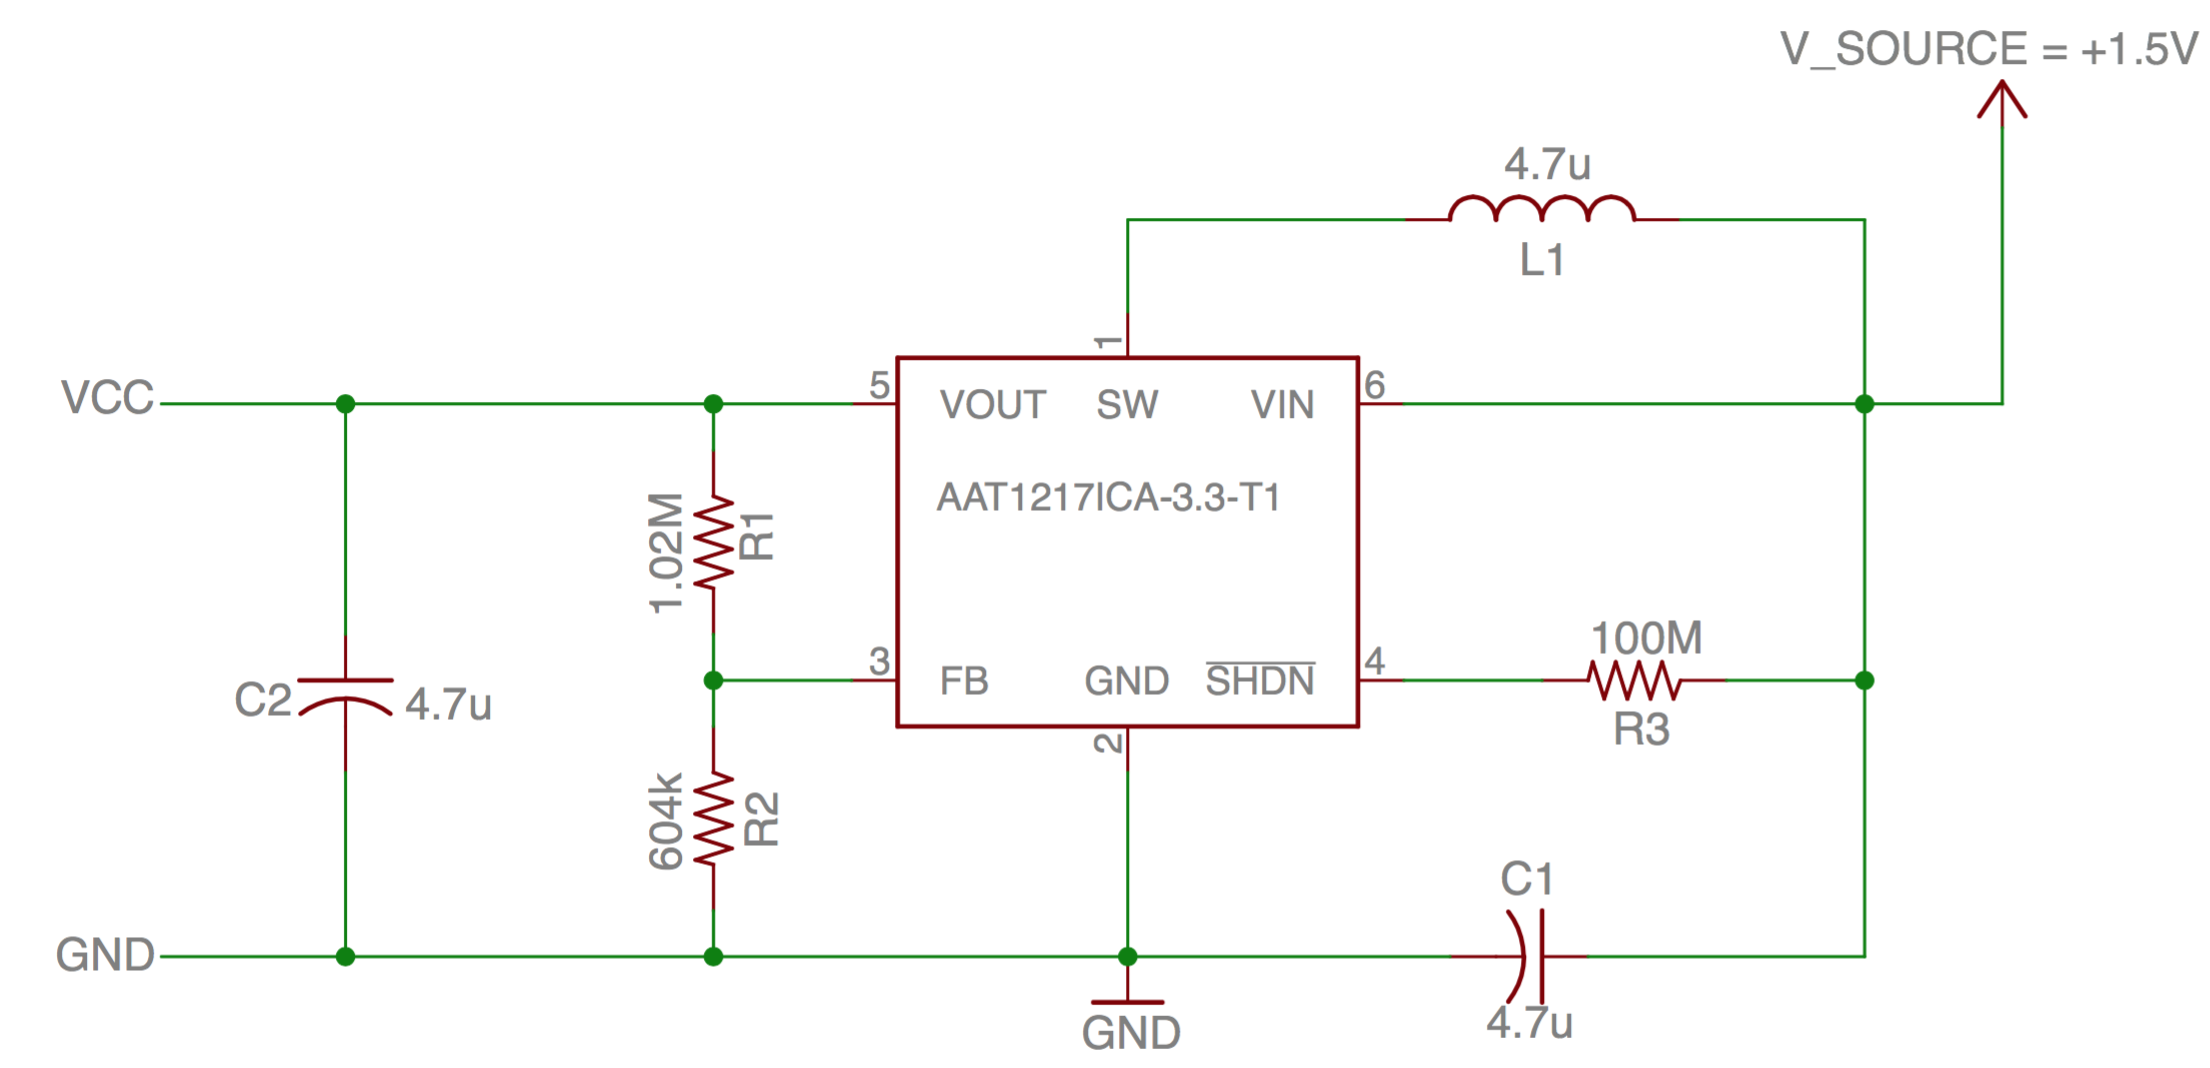
\includegraphics[scale=0.35]{Voltage_Converter_Schematic.png}
	\caption{AAT1217 Circuit Schematic\label{fig:voltage-converter-schematic}}
\end{figure}

\begin{figure} [H]
	\centering
	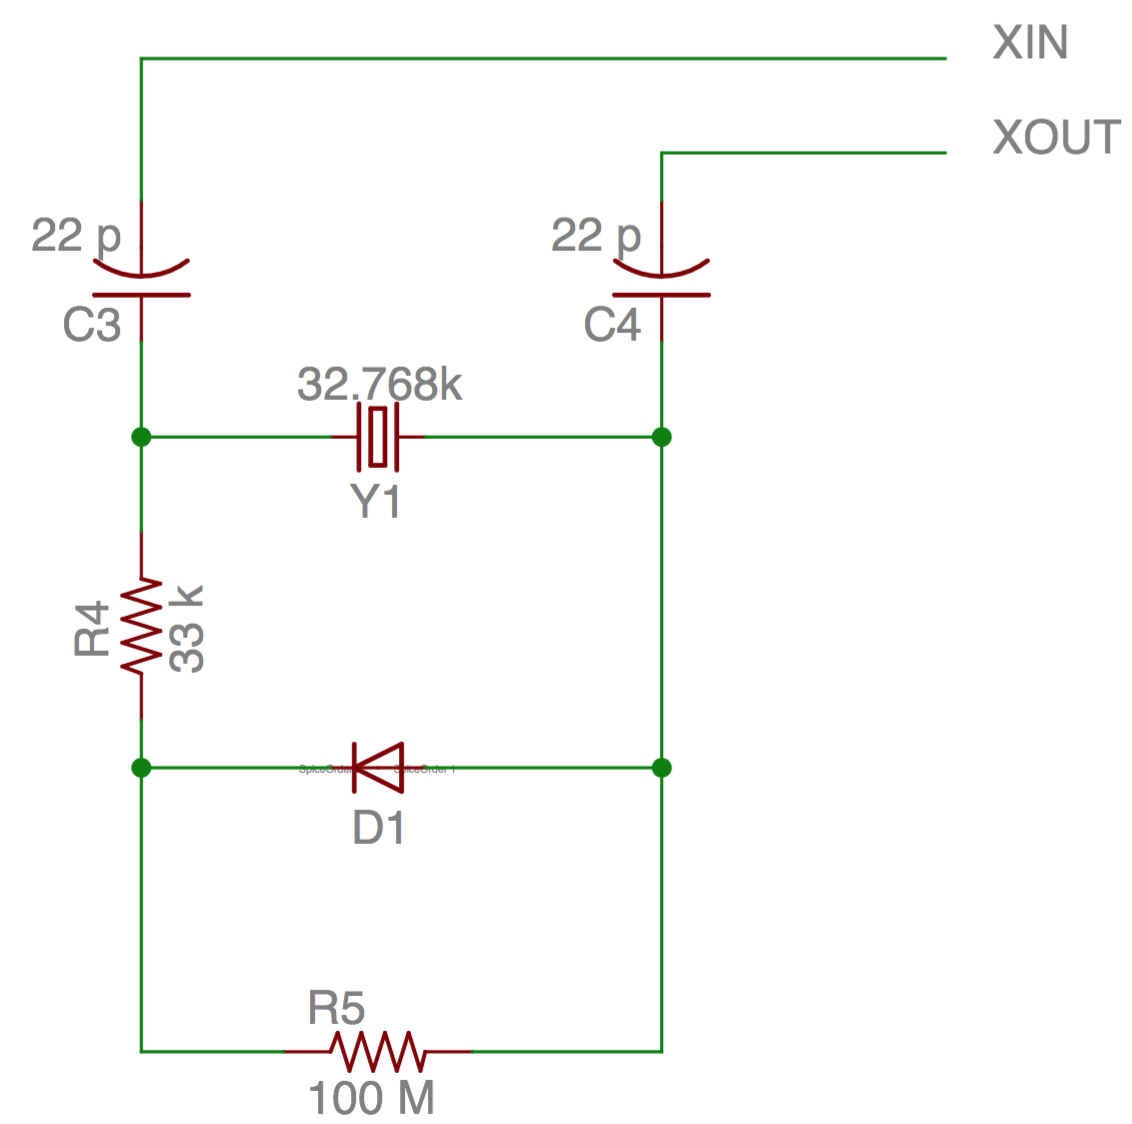
\includegraphics[scale=0.35]{Crystal_Oscillator_Schematic.png}
	\caption{Crystal Oscillator Real Time Clock Circuit Schematic\label{fig:crystal-oscillator-schematic}}
\end{figure}

\begin{figure} [H]
	\centering
	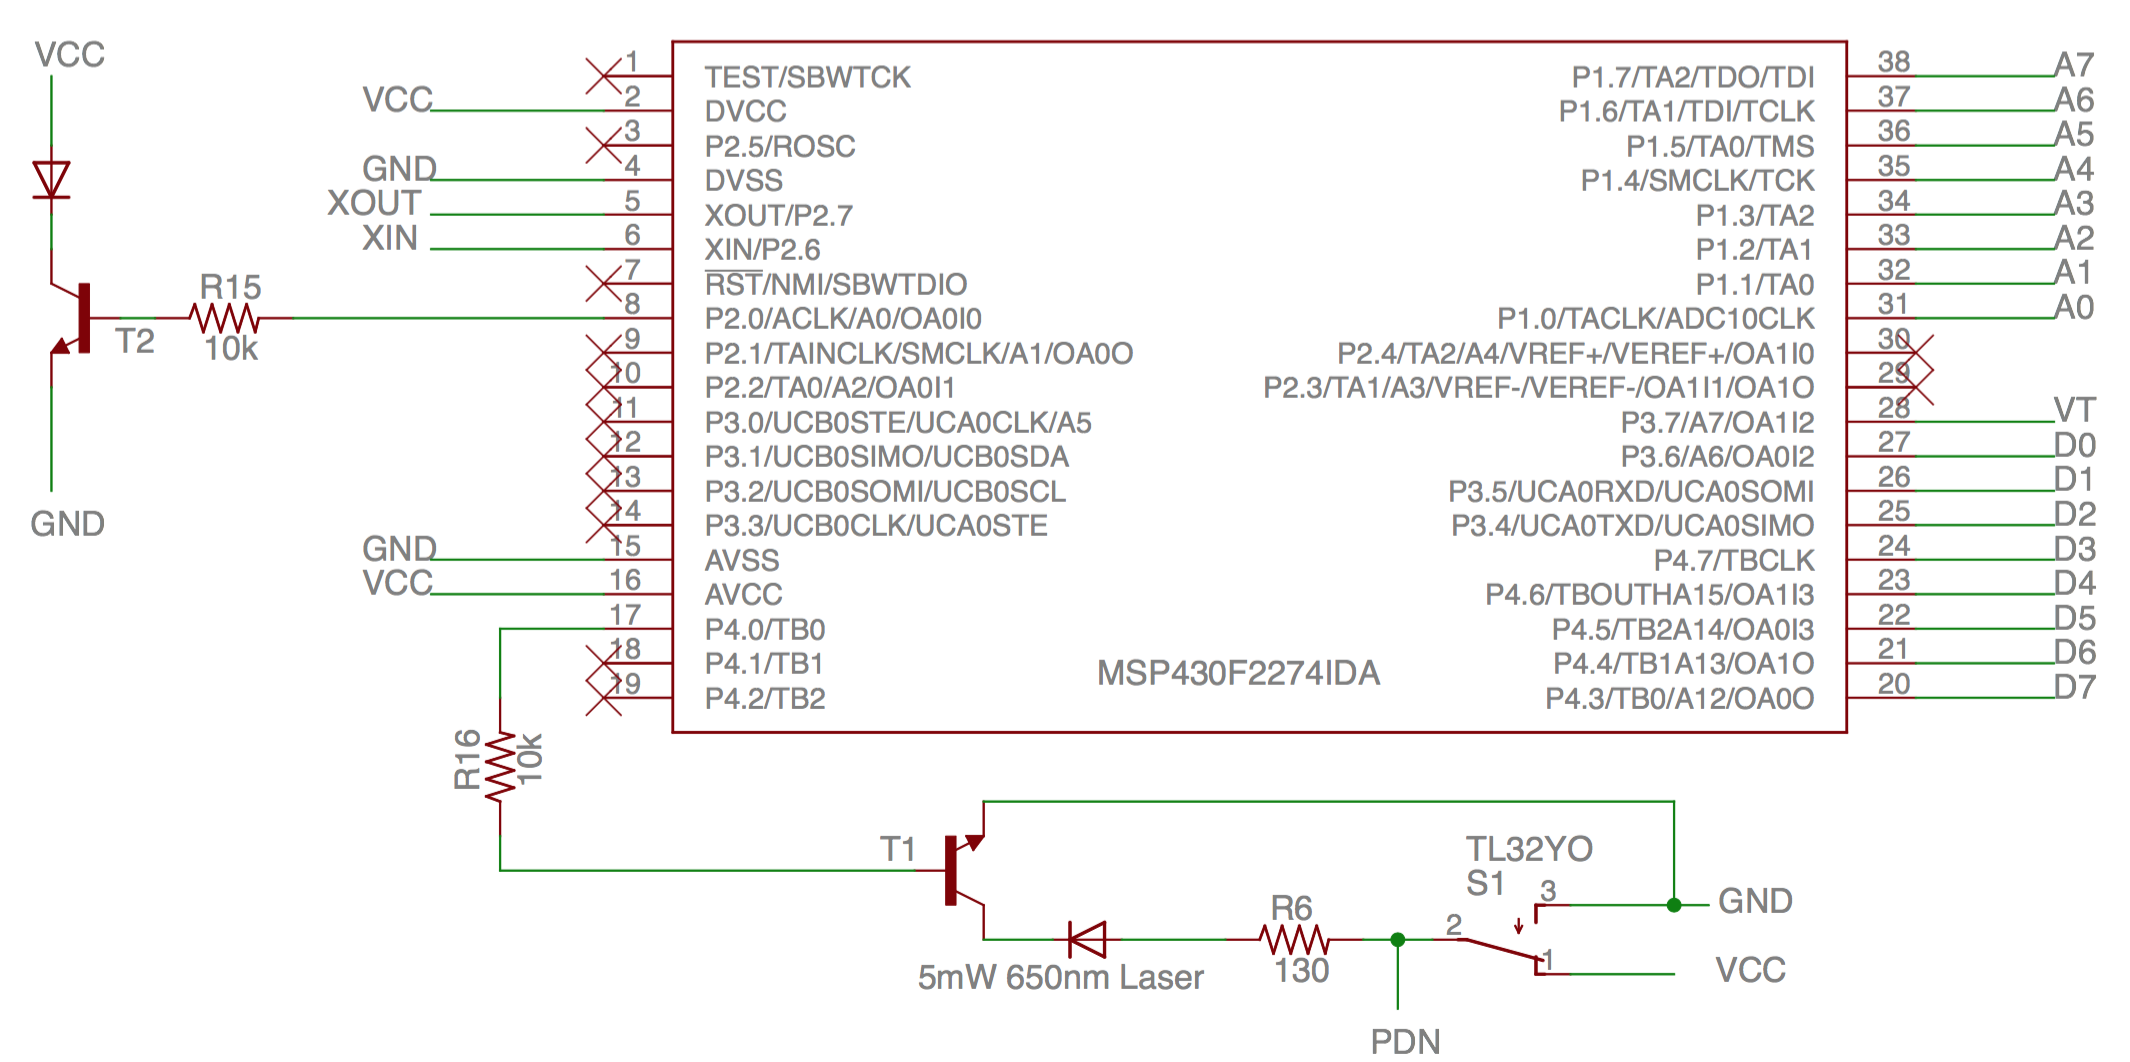
\includegraphics[scale=0.43]{MCU_Laser_Schematic.png}
	\caption{MCU and Laser Transmitter Circuit Schematic\label{fig:mcu-laser-schematic}}
\end{figure}

\begin{figure} [H]
	\centering
	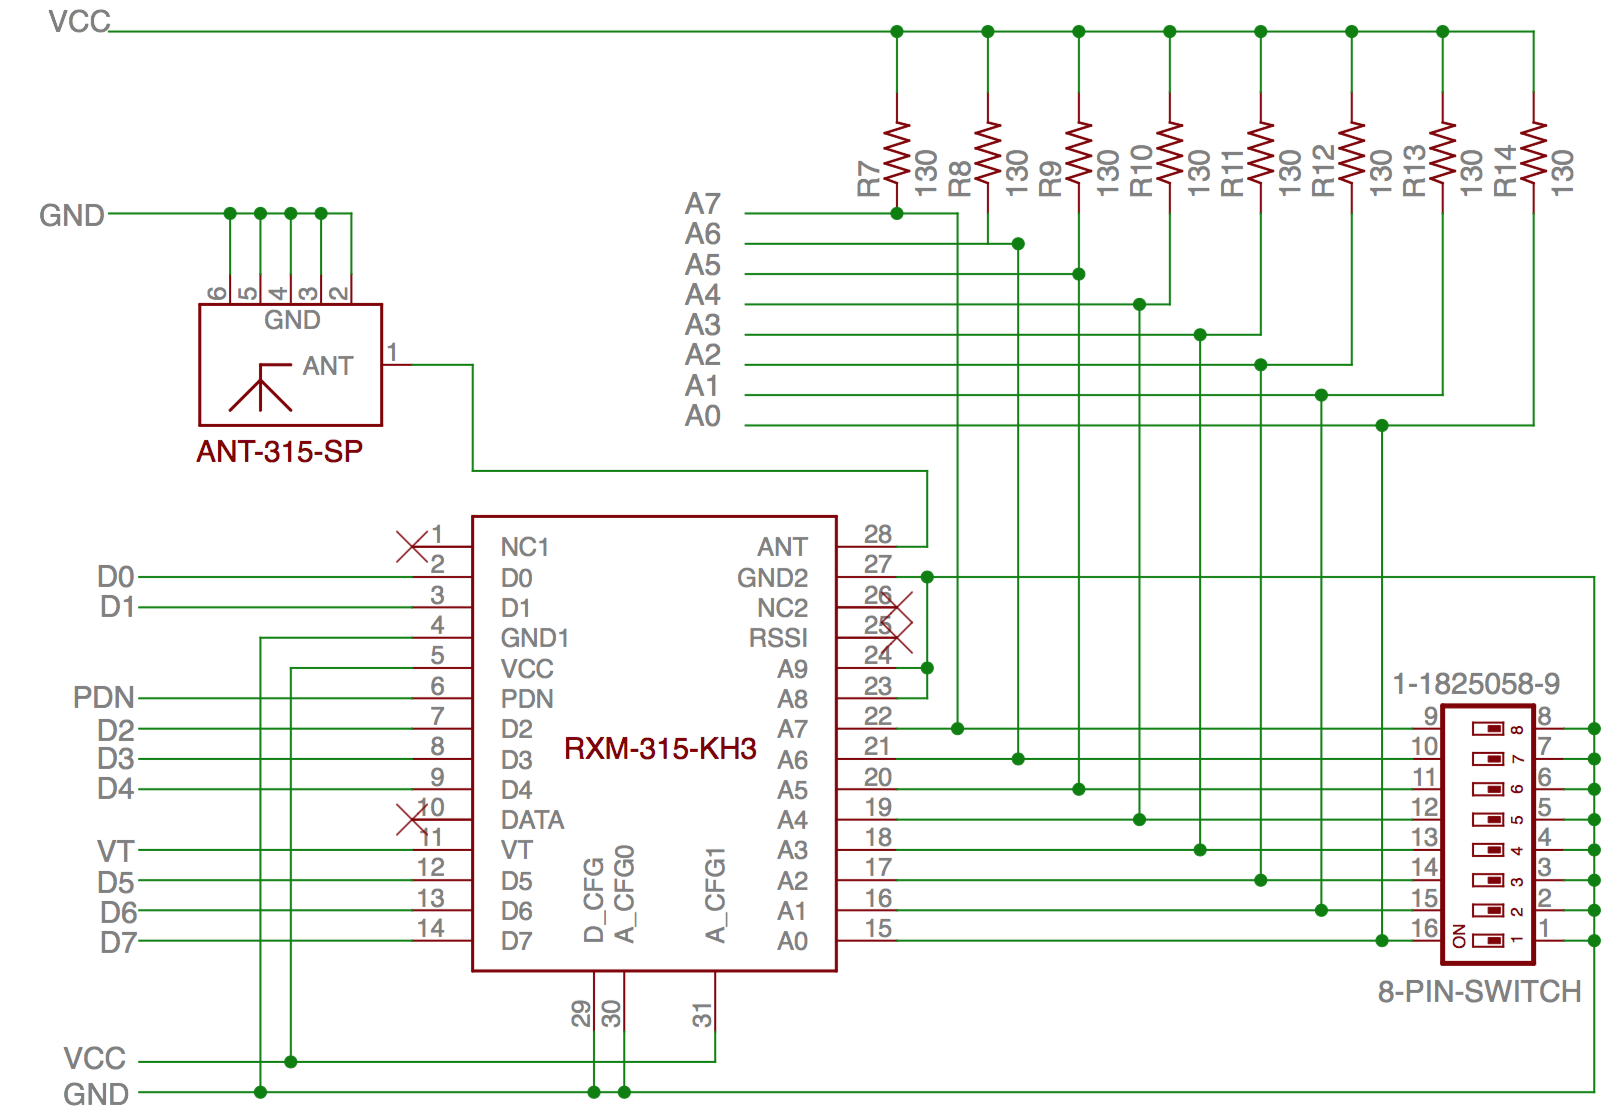
\includegraphics[scale=0.5]{RF_Receiver_Decoder_Schematic.png}
	\caption{RF Receiver/Decoder and 8-Pin DIP Switch Schematic\label{fig:rf-receiver-decoder-schematic}}
\end{figure}


\subsubsection{Friendly Target Unit}

\subsection{Software Flowcharts / Functionality}
\subsubsection{System Flow}
This section is to explain the flow of events in the system as a whole as well as each the friendly interrogator subsystem and the friendly target subsystem. The below diagram is a flowchart representing the events that occur to identify a target as friendly.

\begin{figure} [H]
	\centering
	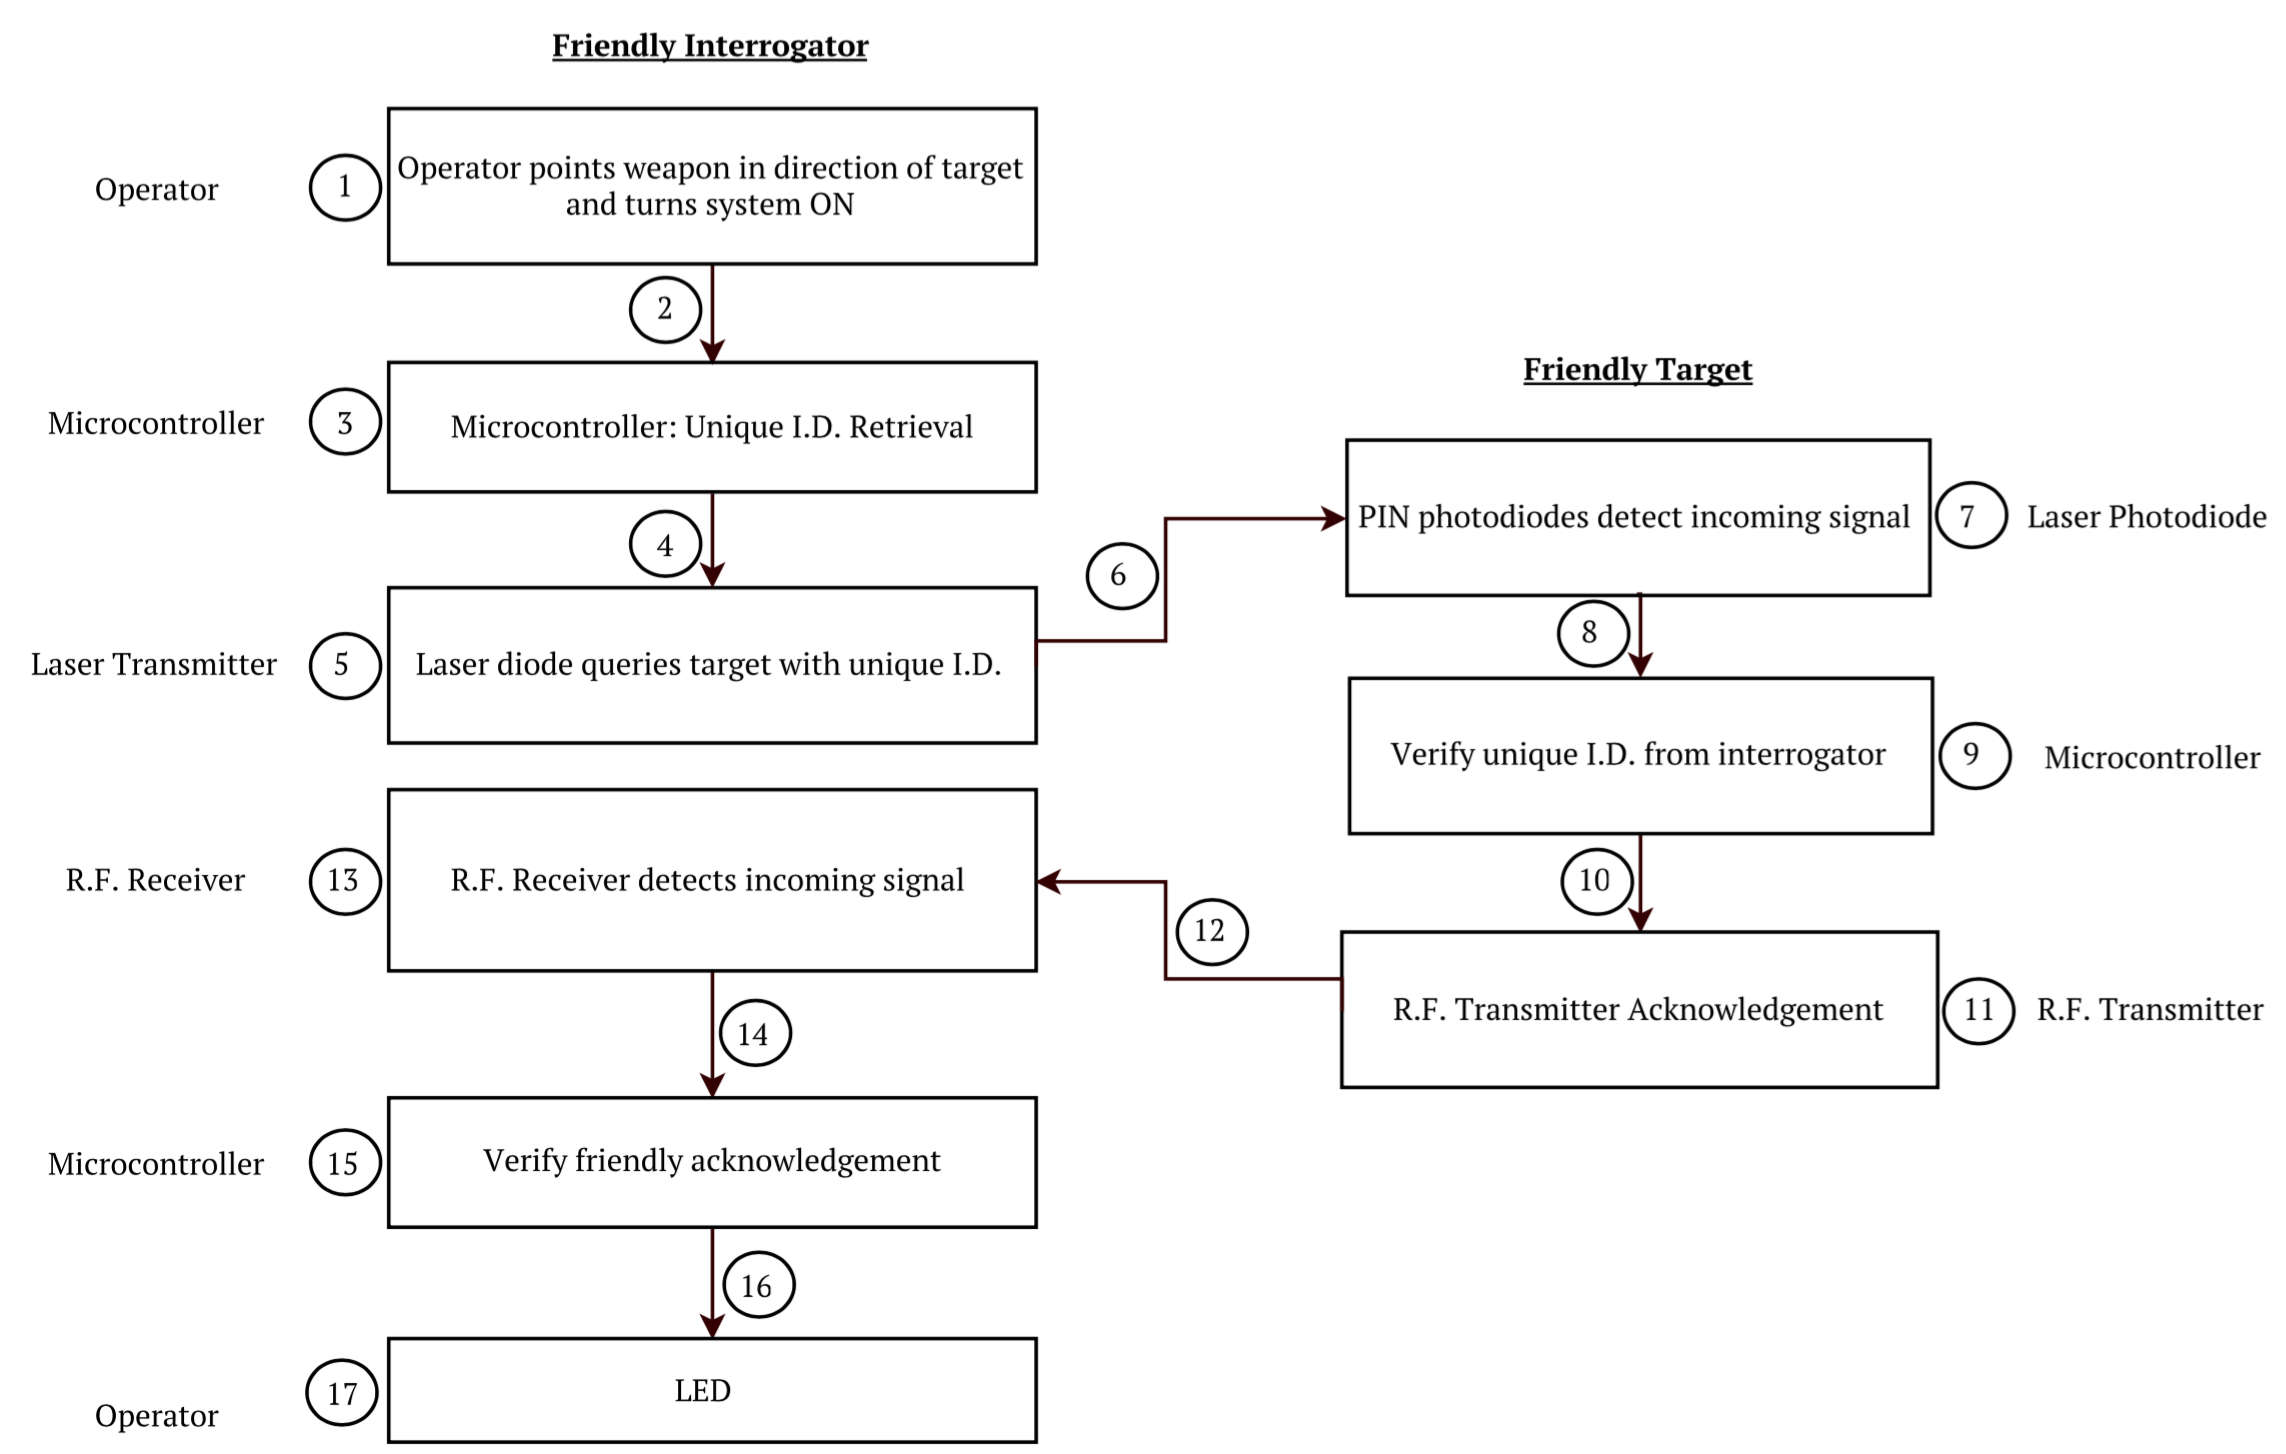
\includegraphics[scale=0.4]{Functional_Flowchart.png}
	\caption{Flowchart for Functionality\label{fig:circuit-schematic}}
\end{figure}

The left side of this diagram are all events that occur within the friendly interrogator unit, and the right side represents all of the events that occur on the friendly target side. This flow diagram also assumes that both the interrogator operator and the friendly target operator have powered on their respective units.

\subsubsection{Friendly Interrogator Software Flow}
The software on the MCU on the friendly interrogator unit will follow a very simple flow. The MSP430F2274 contains 16 registers of which 4 are protected and 12 are general purpose registers:
\begin{itemize}
	\item R0 - program counter
	\item R1 - stack pointer 
	\item R2 - status register
	\item R3 - constant generator
	\item R4 - R15 - general purpose registers
\end{itemize}

Using these 12 general purpose registers the team can accomplish the task 

\subsection{Numerical Analysis and Simulations/Plots} \label{section-simulations-calculations}

\subsubsection{Calculations}
\normalsize\textbf{Power Module (Friendly Interrogator Unit)} \\
The following section is intended to backup the design choices made for the power module on the friendly interrogator first shown in section \ref{section-friendly-interrogator-design}.

The team placed a strict requirement (shown in section \_\_\_) regarding the operation time of the friendly interrogator unit (at 8 hours of operation time $\pm$ 5\% \hl{verify}).

In order to select parts that satisfied this requirement, the active current consumption on the entire unit must first be calculated. The main power consumption modules on board the friendly interrogator unit are the MSP430F2274, the 5mW 635nm TTL laser transmitter, and the Linx KH3 R.F. receiver. These values were received from each of the respective datasheets. The following table displays the active current consumption of each unit. 


\begin{table}[htbp]
	\centering
	\begin{tabular}{c|c|c}	% ccccccc indicates 7 center aligned columns
		\toprule	% top separator
		Module & Active Current Consumption & Standby Current Consumption\\
		\midrule
		MSP430 & 270 $\mu$A & 0.1 - 0.7 $\mu$A\\ 
		Linx KH3 R.F. Receiver & 5.9 mA & 0 mA\\
		5 mW Laser & 25 mA (max) & 0 mA \\
	\bottomrule	% bottom separator
	\end{tabular}%
	\caption{Notable Datasheet Values for Linx 315 MHz LR R.F. Receiver}
	\label{tab:table2}	% this is the label given to the table that can be referenced using \ref{tab:Exp1Part1_7}
\end{table}%

Because the R.F. receiver and the 5mW laser will only be powered when the operator designates, the standby current consumption of these units will be 0.

Therefore, with this information, the maximum possible active current consumption will be:
\begin{center}{I\textsubscript{Total} = $270 \mu A + 25 mA + 5.9 mA + 0.7 \mu A$}\end{center}

Assuming the team uses a standard Alkaline AA 1.5V Battery, these typically produce anywhere from 1800mAh to 2500 mAh \hl{insert reference here}. Therefore, the average of these two values will be used as the capacity of the battery: 2150 mAh. Since all of the components being used requires 3.3V, this battery must be fed into a voltage step-up converter as stated previously. The team is using the AAT1217 step-up converter this boosts the voltage up from 1.5V to 3.3V with a ~75\% efficiency \hl{insert reference here}.

Using energy conservation laws, the equivalent capacity can be determined after stepping this voltage up from 1.5V to 3.3V. Since Energy = Power * time, we can use a ratio of the energy produced per hour of the standard alkaline battery to the output voltage of the converter. This calculation can be shown below:

\begin{center} 
$Total Capacity = \frac{P_\textrm{battery}* time *  V_\textrm{battery}} {V_\textrm{converter-output}} * Converter Efficiency$

$ Total Capacity = \frac{2150 mAh *  1.5V} {3.3V} * 75\% = 732.95 mAh * 0.75 =$ \textbf{14.95 hr active use} 
\end{center}

This result shows that a single standard alkaline AA 1.5V disposable battery will be more than sufficient enough to satisfy the requirements of 8 hours of active use time.

\normalsize\textbf{Antenna-to-Receiver and Antenna-to-Transmitter PCB Impedance Matching} \\
The input impedance of both the Linx R.F. receiver, transmitter and antenna are all 50 $\Omega$. Therefore, in order to match this impedance on the line that goes from the receiver/transmitter chip to the antenna chip, the width must be calculated on the PCB trace. 

Figure \ref{fig:pcb-trace} shows all variables that affect the impedence of a PCB trace. 

\begin{center}
	$T $ = trace thickness (in mils) \\
	$W$ = trace width  (in mils) \\
	$H$ = heigh of substrate (in mils) \\
	$\epsilon$ = dielectric constant of material
\end{center}

\begin{figure} [H]
	\centering
	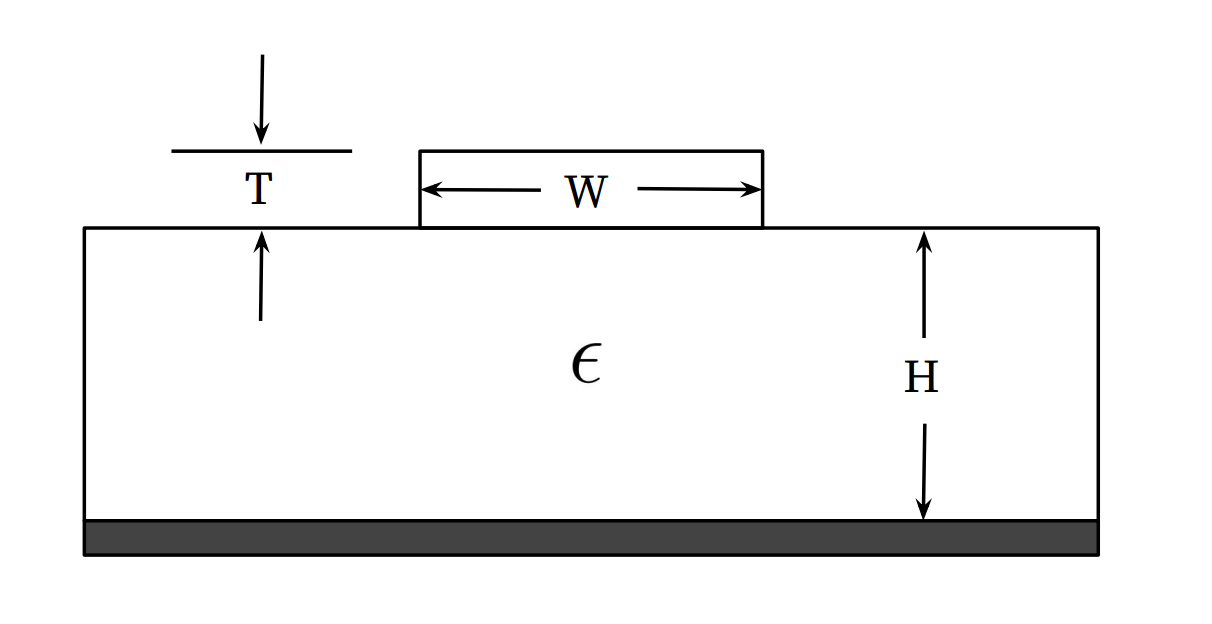
\includegraphics[scale=0.3]{PCB_Trace_Figure.png}
	\caption{PCB Microstrip Impedence Variables\label{fig:pcb-trace}}
\end{figure}

The equation to calculate the impedance is as follows:
\begin{center}
\large$Z = \frac{Z_0}{2\pi*\sqrt{2}*\sqrt{\epsilon+ 1}} * ln\left(1 + 4*\frac{H}{w_{eff}} * \left(X_1 + X_2 \right )\right )$
\end{center}
where
\begin{center}
	\large $W_{eff} = W + \left(\frac{T}{\pi}\right)*ln\left \{\frac{4*e}{\sqrt{\left(\frac{T}{H}\right)^2 + \left (\frac{T}{W*\pi + 1.1*T*\pi }  \right )^{2}}} \right \}$
	
	\vspace{2.5mm}
	
	$X_1 = \frac{4*\left( 14*\epsilon +8\right)}{11*\epsilon} * \left(\frac{H}{W_{eff}} \right)$
	
	\vspace{2.5mm}
	
	$X_2 = \sqrt{16*\left(\frac{H}{W_{eff}} \right )^2 * \left(\frac{14*\epsilon+8}{11*\epsilon} \right )^2 * \left(\frac{\epsilon + 1}{2*\epsilon} \right ) * \pi^2}$
\end{center}

The ECE parts shop uses 1 oz copper trace and FR4 board material as its substrate \hl{insert reference}. Assuming these properties have not changed at the time of this design review, then the following values can be used for T, H, Z, $Z_0$ and $\epsilon$ :
\begin{center}
	$Z_0 =$ impedence of free space $\approx$ 120 $\pi \Omega$ \\
	$T = 1.4 $mils\\
	$H =1.6 $mm\\
	$\epsilon = 1.4$ \\
	$Z = 50 \Omega$
\end{center}
The result after plugging in each respective value and solving for W, is that the PCB trace must be \textbf{3.23 mm} wide going from each R.F. module to the antenna.


\normalsize\textbf{R.F. Transmitter/Receiver Range} \\
The range of the R.F. transmitter and receiver is required to reach a distance of 300 meters. The range in kilometers is a function of the following variables:
\begin{center}
$P_T$ = Transmitter Power (dBm) \\
$A_g$ = Total Antenna Gain (dB) \\
$C_l$ = Connection Loss (dB) \\ 
$G_{tot}$ = Total Gain (dB) \\
$R$ = Receiver Sensitivity (dBm) \\
$L$ = Transmission Path Loss (dB) \\
$f_{MHz}$ = Frequency in MHz \\
\end{center}

Transmission Path Loss is the sum of all the antenna R.F. gains and deduction of all possible losses. Assuming a perfect system on the ground without any interference the following equation can be used to calculate the path loss in a transmission:
\begin{center}
	$L = P_T + (A_g - C_l)$
\end{center}
This equation can be used in conjunction with the following equation to calculate the total range in kilometers:
\begin{center}
	\large
	$d_{TX->RX} = 10^{\left( \frac{L - 32.45 -20*log(f_{MHz})}{20}\right)}$
\end{center}
The following values were used in this range calculation:
\begin{center}
$P_T$ = +4dBm \\
$A_g$ = 2.15 dBi (quarter-wave monopole) \\
$C_l$ = 0 dB \\ 
$G_{tot}$ =  2.15dB\\
$R$ = -116 dBm \\
$L$ =  120.15\\
\end{center}
Plugging in these values to the equation stated before, the team received a range of \textbf{77.03 km} which well surpasses the requirements of 300 m. \\

\normalsize\textbf{Power Module (Friendly Target Unit)} \\

\normalsize\textbf{Laser Diode} \\
\hl{Put lens equations, ref tolerance analysis}

\subsubsection{Simulations/Plots}
\hl{INSERT PLOTS/ANY SORT OF ANALYSIS HERE}


%SECTION - Requirements and Verification
\section{Requirements and Verification}
\hl{UPDATE THIS TABLE-maybe reference an appendix in the back?}
\begin{figure} [H]
	\centering
	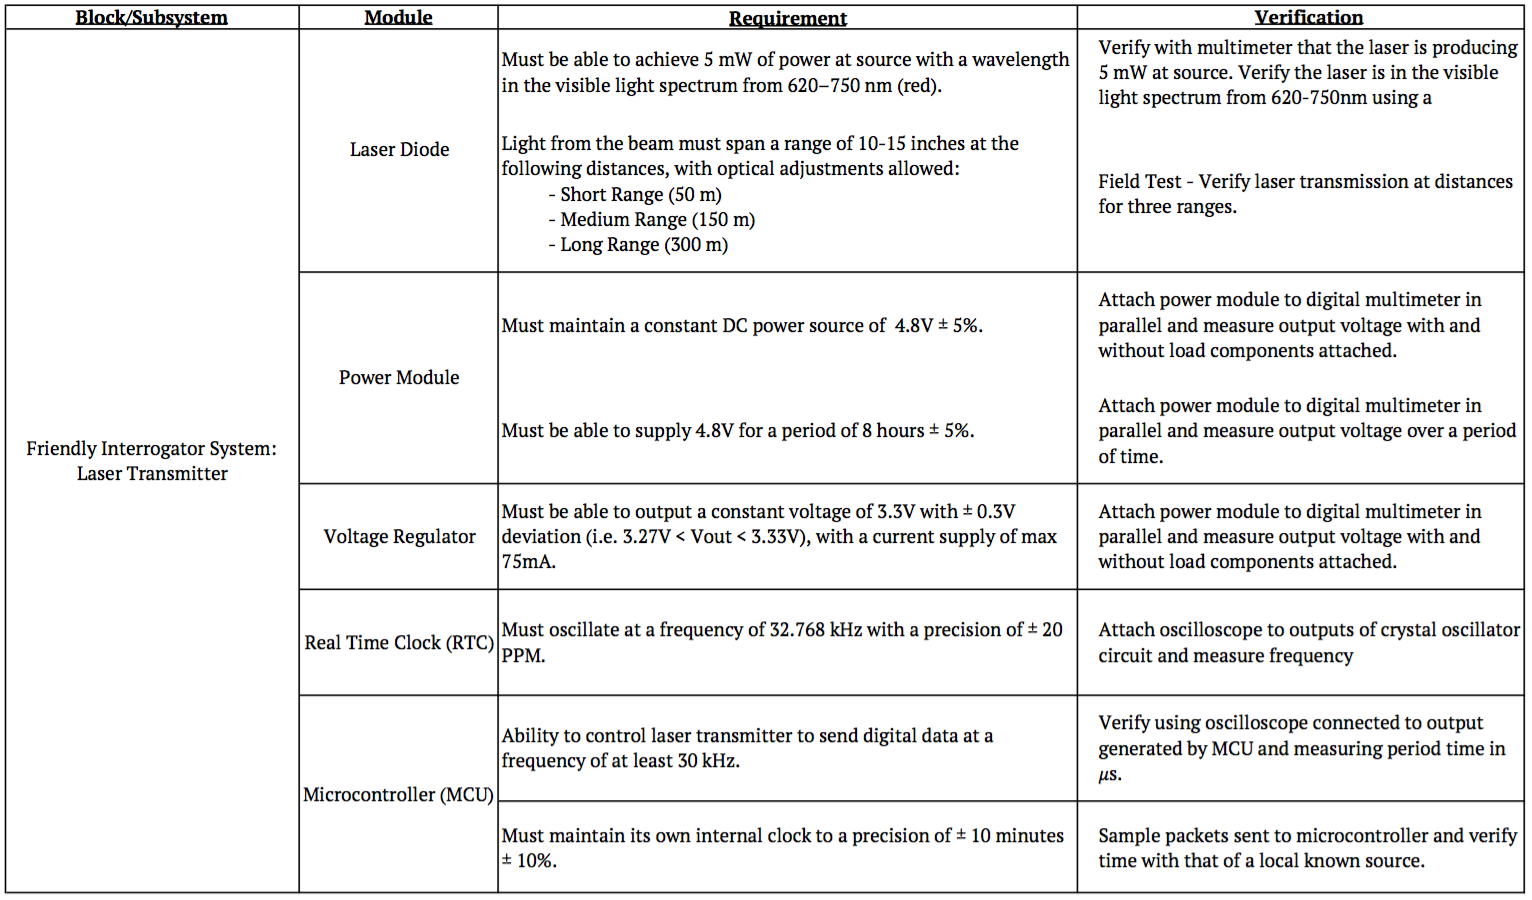
\includegraphics[scale=0.3]{Requirements.png}
	\caption{Requirements/Verification for Laser Transmitter System\label{fig:requirements}}
\end{figure}
\subsection{Tolerance Analysis} \label{section-tolerance-analysis}
The inherent limitations of laser power for safety means that the performance is in the hands of the photodiode. The starting point for selection criteria was to choose a photodiode type. There are three main photodiode types: normal, PIN, and Avalanche; the team chose PIN photodiodes as they have a high sensitivity and speed. A normal photodiode would not be sensitive enough to register a wide divergence $5mW$ laser, and an Avalanche photodiode requires high voltage. 

The next selection criteria is the material with which the photodiode is made. This includes materials such as Si, InGaAs, and InA. The optimum wavelength is dependent on the material selection.

With photodiodes, Noise-equivalent Power (NEP) is a measure of the incident power required to generate a response signal equal to the noise level of a detector system. Detectivity is the reciprocal of the NEP normalized for the active area of the photodiode.\textsuperscript{\cite{Microphotonics}}. The best photodiode, then, will have the highest detectivity for the visible wavelength.  

\begin{figure} [H]
	\centering
	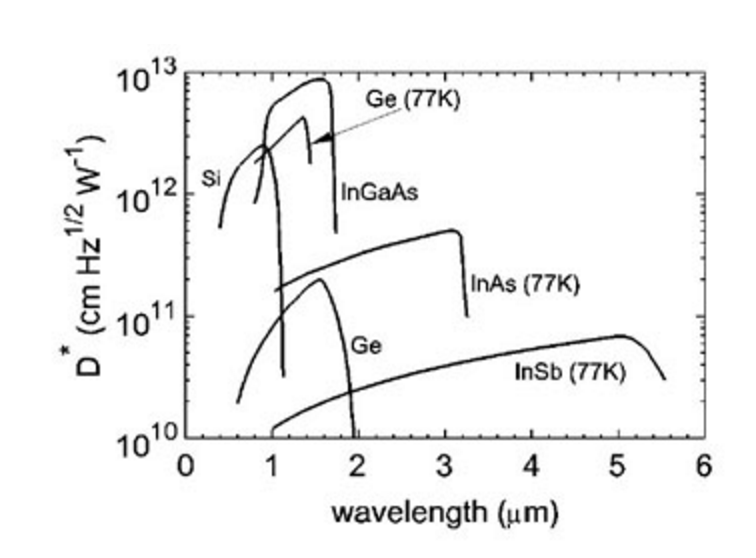
\includegraphics[scale=0.4]{detectivity-table.png}
	\label{fig:detectivity-table}
	\caption{Specific Detectivity for Photodetector Materials \textsuperscript{\cite{Optical}} \label{fig:detectivity-table}}
\end{figure}

Figure \ref{fig:detectivity-table} illustrates the specific detectivity ranges of photodiodes. The interrogation laser is in the visible range; therefore, the matching photodiode is of type Si. Using this type of photodiode, the detectivity is between $10^{10}$ and $10^{13}$ $\frac{Hz^{\frac{1}{2}}}{W}$. The following calculations will use a conservative value, $10^{12} \frac{Hz^{\frac{1}{2}}}{W}$, as the detectivity. In realty, because the wavelength is less than \SI{1}{\micro\meter}, the detectivity is somewhere between $10^{12}$ and $10^{13}$ $\frac{Hz^{\frac{1}{2}}}{W}$

The equation for NEP from detectivity, $D^*$, and photodiode active area, $A$,  is 
\begin{center}
	{\large $NEP = \frac{\sqrt{A}}{D^*}$}  $[\frac{W}{Hz^{1/2}}]$
\end{center}

The incident irradiance, $E_i$, to cancel noise is
\begin{center}
	{\large $E_i = \frac{NEP * \sqrt{f}}{A} = \frac{\sqrt{Af}}{AD^*} = \frac{f}{D^*\sqrt{A}}$} $[\frac{W}{m^{2}}]$
\end{center}

The NEP measures the incident irradiance to cancel the noise on the photodiode. To register a signal on the MCU, the incident irradiance must be higher than the noise. To be conservative, define the required incident irradiance as 
\begin{center}
	{\large $E_{req} = 2E_i$} $[\frac{W}{m^{2}}]$
\end{center}

Multiplying the area of the laser's spot by the required incident irradiance at the photodiode gives the necessary power. Thus, the radius of the spot in terms of the power of the laser and required incident irradiance at the photodiode is 
\begin{center}
	{\large $r = \sqrt{\frac{P}{\pi E_{req}}}$} $[m]$
\end{center}

Note that the power contained in the laser's spot does not depend on distance from the source, as atmospheric reflection is negligible at $300 m$.

The radius, in terms of the detectivity, frequency, and sensor active area is
\begin{center}
	{\large $r = \sqrt{\frac{PD^*\sqrt{A}}{2 \pi f}}$} $[m]$
\end{center}

The proposal listed $0.8382 m$ as the ideal radius of the laser's spot. Unfortunately, with the $5mW$ red laser, this would require a sensor with a massive active area. The largest sensor the team could find, at a reasonable price, has a $100 mm^2$ active area. 

For the $100 mm^2$ active area photodiode operating at $650 nm = 4.61219 × 10^{14} Hz$ 
\begin{center}
	$r = 0.608721 m \approx 61 cm$
\end{center}

Refining the proposal requirements, the team has set a new requirement of a $50 cm$ laser spot radius, making the diameter of the beam $1m$ at distances of $50m, 150m,$ and $300m$ with optical adjustment. 

Capturing these requirements, the team must transmit a signal to a photo-detector at the following ranges:
\begin{itemize}
	\item Short Range (0 - 50 m)
	\item Medium Range (50 - 150 m)
	\item Long Range (150 - 300 m)
\end{itemize}

The team should then verify that the signal was received. Furthermore, the team should verify that the signal spans the width of a human chest. More concretely, that a sighted-in laser transmitter can be aimed at any point within $50 cm$ of the receiver and still register the transmitted signal. 

Test Procedure:

\begin{itemize}
	\item Mount the receiver 300 m downrange of the transmitter
	\item Aim the laser transmitter directly at the receiver, using a mount (like a vice grip) to keep it stable. 
	\item Verify the signal is received via the probe point on the PCB
	\item Aim and verify the signal is also received when aiming 25 cm to the right, top, and bottom of the receiver. 
	\item Repeat these steps for 50 m and 150 m. 
\end{itemize}



\subsection{Safety} \label{section-safety-ethics}
\normalsize\textbf{Laser Diode} \\
As stated previously, the proposal requirements would have required a $20mW$ IR laser. However, in the State of Illinois, a 20mW laser is considered a Class 3B laser and must be registered with the Division of Nuclear Safety in the Illinois Emergency Management Agency. This would have required the team to file the correct paperwork and pay a registration fee of \$50. This paperwork would have likely caused delays in receiving parts and construction of this project. A 20 mW laser would have also needed much more pre-caution and safety mitigations than a much less powerful laser.

For the reasons stated above, the team will instead use a $5mW$ visible red laser. $5mW$ visible lasers have a low chance of injuring the eye, as the blinking reflex will save a victim from permanent damage; as opposed to IR lasers which can go unnoticed for several seconds. 

The following is a calculation for the nominal ocular hazard distance (NOHD) of our laser, as defined by the ANSI Standard \cite{ANSI}.

The maximum permissible exposure (MPE), as defined by the ANSI Standard \cite{ANSI} is the highest power or energy density of a light source that is considered safe, i.e. that has a negligible probability for creating damage. This MPE for a pulsing laser is calculated as the minimum of the following three rules:

\begin{enumerate}
	\item Any single pulse in the train must not exceed the MPE for the pulse exposure time.
	\item The exposure from any group of pulses delivered in time T must not exceed the MPE for
	time T, where T is 0.25 seconds (from the blinking reflex), for a visible laser. 
	\item For thermal injury, the exposure for any single pulse within a group of pulses must not
	exceed the single-pulse MPE multiplied by a multiple-pulse correction factor
\end{enumerate}

The laser will pulse at a rate of 40 kHz. Assuming at most a 50\% duty cycle, each pulse will be of max length $1.25*10^{-5} s$. The divergence of the beam is smallest for the longest range; a lower divergence is more restrictive in terms of safety, so this calculation uses $300m$. The divergence of the beam for 300m is 2.79 mrad and the beam waist is approximately $4 mm$. \\

Following the ANSI Standard \cite{ANSI}, the Rule 1 calculation is 

{\large $5*10^{-3}*(\frac{2.79}{1.5})  = 0.0093 \frac{J}{m^2}$ }\\

The Rule 2 calculation is

{\large $\frac{18(.25^{0.75})(\frac{2.79}{1.5})}{.25*40000} = 0.0011837 \frac{J}{m^2}$ }\\

The Rule 3 calculation is

{\large $(.25*40000)^{0.25} * 5*10^{-3}*(\frac{2.79}{1.5}) = 0.093 \frac{J}{m^2}$ }\\

The most restrictive of all the rules is Rule 2, which gives us an MPE of $0.0011837 \frac{J}{m^2}$.

At $5mW$ with a pulse width of $1.25*10^{-5}$, the power of the laser is $6.25*10^{-8} J$. 

The NOHD is defined as

{\LARGE $ \frac{\sqrt{\frac{4 * P}{\pi * MPE}} - 2w}{\theta}$}

Where P is the power of the beam ($6.25*10^{-8} J$) and $w$ is the waist of the beam ($1mm$). This gives an NOHD of 

{\Large$ \frac{\sqrt{\frac{4 * 6.25*10^{-8}}{\pi * 0.0011837}} - 2(0.004)}{0.00279} = 0.0713 m $}

The team will avoid eye damage by not working with their eyes inside of 8 cm from the laser. If it is necessary to get this close to the laser, the team will wear eye protection or simply power off the laser. 


\subsection{Ethical Issues}
This project has several ethical issues that can be addressed by the IEEE Code of Conduct. Specifically, numbers 1, 2, 3, 5, 6, 7, and 9 are the most important items that pertain to the Infantry I.F.F. System the team is building this semester. 
\begin{enumerate}
\item to accept responsibility in making decisions consistent with the safety, health, and welfare of the public, and to disclose promptly factors that might endanger the public or the environment;
\item to avoid real or perceived conflicts of interest whenever possible, and to disclose them to affected parties when they do exist;
\item to be honest and realistic in stating claims or estimates based on available data;  
\skipitems{1}
\item to improve the understanding of technology; its appropriate application, and potential consequences;  
\item to maintain and improve our technical competence and to undertake technological tasks for others only if qualified by training or experience, or after full disclosure of pertinent limitations;  
\item to seek, accept, and offer honest criticism of technical work, to acknowledge and correct errors, and to credit properly the contributions of others;  
\skipitems{1}
\item to avoid injuring others, their property, reputation, or employment by false or malicious action;  
\end{enumerate}

%SECTION - Cost and Schedule
\clearpage
\section{Cost and Schedule}

\subsection{Cost Analysis}
The labor cost was calculated as follows:

\begin{center}
	Labor Cost = Worker Salary (\$/hour) x 2.5 x Time (Hours) Invested In Project
\end{center}

\hl{COMPILE PARTS LIST, SUM UP TOTAL, ADD TO LABOR COSTS - SAME AS PROPOSAL}

\subsection{Schedule}
\hl{EDIT SCHEDULE CREATED IN PROPOSAL}


%SECTION - References
\clearpage
\bibliographystyle{IEEE_ECE}
% include the BibTex file here to build reference
\bibliography{Citations}\addcontentsline{toc}{section}{Reference}

\clearpage
\end{spacing}
\end{document}

